% =============================================================================
%  Aircraft Performance Engine -- Methodology Report
%  Author : Mark Barsoum
%
%  Font: Charter.
%  1. Generate the worked examples from the model (from the project folder):
%         python3 report/make_examples.py
%  2. Compile with pdfLaTeX (run twice for the contents and cross-references):
%         cd report && pdflatex performance_model.tex
%  Works on Overleaf with the default pdfLaTeX compiler.
% =============================================================================
\documentclass[11pt,letterpaper]{article}

% ---- Page, font and typography ----------------------------------------------
\usepackage[top=1in, bottom=1in, left=1in, right=1in, headheight=14pt]{geometry}
\usepackage[OT1,T1]{fontenc}
% Code font: Computer Modern Typewriter in OT1, which is a scalable Type 1 font everywhere
\makeatletter\expandafter\let\csname orig@tt\expandafter\endcsname\csname ttfamily \endcsname\expandafter\def\csname ttfamily \endcsname{\fontencoding{OT1}\orig@tt}\makeatother
% Charter text with matching Charter math. XCharter + newtxmath is the best
% pairing (standard on Overleaf / full TeX Live); fallbacks keep it compiling
% on smaller installations.
\IfFileExists{XCharter.sty}{%
  \usepackage[osf=false]{XCharter}%
  \usepackage[charter,vvarbb,scaled=1.05]{newtxmath}%
}{%
  \IfFileExists{mathdesign.sty}{%
    \usepackage[bitstream-charter]{mathdesign}%
  }{%
    \usepackage{charter}%
  }%
}
\usepackage{microtype}
\usepackage{setspace}
\setstretch{1.1}

% ---- Mathematics, units, tables, figures ------------------------------------
\usepackage{amsmath,amssymb}
\numberwithin{equation}{section}
\usepackage{siunitx}
\sisetup{group-separator={\,}, group-digits=integer, group-minimum-digits=4, per-mode=symbol, mode=text}
\usepackage{booktabs,tabularx,longtable,array}
\usepackage{graphicx}
\usepackage{float}
\usepackage[font=small, labelfont=bf, labelsep=period, skip=6pt]{caption}
\usepackage[dvipsnames]{xcolor}
\usepackage{enumitem}
\setlist{itemsep=2pt, topsep=4pt, leftmargin=1.6em}
\usepackage{lastpage}
\usepackage[most]{tcolorbox}

% ---- Colours ----------------------------------------------------------------
\definecolor{navy}{HTML}{1F3A5F}
\definecolor{navylight}{HTML}{E8EDF4}
\definecolor{ink3}{HTML}{6B6A64}

% ---- Prominent headings ------------------------------------------------------
\usepackage{titlesec}
\titleformat{\part}[display]
  {\centering\color{navy}\bfseries}
  {\Large PART \thepart}{0.6em}
  {\Huge}[\vspace{0.6em}{\color{navy}\titlerule[1.5pt]}]
\titlespacing*{\part}{0pt}{2.5in}{1.5em}
\titleformat{\section}
  {\color{navy}\LARGE\bfseries}
  {\thesection}{0.8em}{}
\titlespacing*{\section}{0pt}{2.0em}{0.9em}
\titleformat{\subsection}
  {\color{navy}\Large\bfseries}
  {\thesubsection}{0.7em}{}
\titlespacing*{\subsection}{0pt}{1.5em}{0.6em}
\titleformat{\subsubsection}
  {\normalsize\bfseries}
  {\thesubsubsection}{0.6em}{}
\titlespacing*{\subsubsection}{0pt}{1.1em}{0.4em}
\setcounter{secnumdepth}{3}
\setcounter{tocdepth}{2}

% ---- Header and footer --------------------------------------------------------
\usepackage{fancyhdr}
\pagestyle{fancy}
\fancyhf{}
\fancyhead[L]{\small\itshape Aircraft Performance Engine}
\fancyhead[R]{\small\itshape Methodology Report}
\fancyfoot[L]{\small M.~Barsoum}
\fancyfoot[R]{\small Page \thepage\ of \pageref{LastPage}}
\renewcommand{\headrulewidth}{0.4pt}
\renewcommand{\footrulewidth}{0.4pt}
\fancypagestyle{plain}{\fancyhf{}\renewcommand{\headrulewidth}{0pt}\renewcommand{\footrulewidth}{0pt}}

\usepackage{tocloft}
\renewcommand{\cftsecleader}{\cftdotfill{\cftdotsep}}
\renewcommand{\cftpartfont}{\large\bfseries\color{navy}}
\setlength{\cftbeforesecskip}{4pt}

\usepackage[hidelinks]{hyperref}

% ---- Function boxes ----------------------------------------------------------
\newtcolorbox{funcbox}{enhanced, colback=navylight, colframe=navy, boxrule=0.6pt,
  arc=2pt, left=6pt, right=6pt, top=4pt, bottom=4pt, fontupper=\small}
\newcommand{\func}[2]{\begin{funcbox}\texttt{#1}\\[2pt]{\color{ink3}Returns:} #2\end{funcbox}}
\newcommand{\code}[1]{\textmd{\texttt{#1}}}
\setlength{\cftsubsecnumwidth}{3em}
\newcommand{\src}[1]{[#1]}
\setlength{\parindent}{0pt}
\setlength{\parskip}{0.55em}
\renewcommand{\arraystretch}{1.18}

% Keep headings with their content: start a new page if too little room is left
\usepackage{needspace,etoolbox}
\preto\section{\Needspace{12\baselineskip}}
\preto\subsection{\Needspace{8\baselineskip}}
\preto\subsubsection{\Needspace{6\baselineskip}}

\begin{document}

% =============================================================================
%  Title page
% =============================================================================
\begin{titlepage}
\centering
\vspace*{2.2in}
{\color{navy}\rule{\linewidth}{1.5pt}}\par\vspace{0.6em}
{\LARGE\bfseries\color{navy} Aircraft Performance Engine\par}
\vspace{0.5em}
{\Large\color{navy} Takeoff \& Landing Performance Model\par}
\vspace{0.7em}
{\large Methodology Report: Formulas, Methods and Worked Examples\par}
\vspace{0.4em}
{\color{navy}\rule{\linewidth}{1.5pt}}\par
\vspace{0.6in}
{\normalsize Atmosphere, aircraft, takeoff, Balanced Field Length, landing and runway analysis,\\
organised by Python file and function, with worked examples for the\\
Bombardier Challenger 3500 and the Cirrus SR22T\par}
\vfill
{\large Mark Barsoum\par}
\vspace{0.4in}
{\normalsize October 2026\par}
\end{titlepage}

% =============================================================================
%  Summary
% =============================================================================
\pagenumbering{roman}
\section*{Summary}
\addcontentsline{toc}{section}{Summary}

This report sets out the methodology behind a Python model of aircraft takeoff and landing performance. It does not evaluate the results; it explains, step by step, how they are obtained.

\textbf{Part I} follows the structure of the code. Each section covers one Python file, and each subsection one function: what it takes in, what it returns, the formulas it evaluates and the source of each method. The files build on one another, from unit conversion and the atmosphere, through the aircraft model and the equations of motion, to the takeoff distance, the Balanced Field Length (BFL) with an engine failure at the decision speed $V_1$, the landing distance and the runway checks.

\textbf{Part II} applies the method to two aircraft on the same runway and day: a Bombardier Challenger 3500 twin-engine business jet and a Cirrus SR22T single-engine turbocharged piston aircraft. Every intermediate value is shown with the numbers substituted into the equations of Part I. The worked examples are generated directly from the model by \code{report/make\_examples.py}, so the numbers in the report always match the code.

\newpage
\tableofcontents
\listoffigures
\listoftables
\newpage
\pagenumbering{arabic}

% =============================================================================
\section{Introduction}
% =============================================================================
\subsection{Purpose}
Takeoff and landing performance determines which runways an aircraft can use and at what weight. For transport-category aircraft, the certified takeoff distance is set by the most critical engine-failure case, not only by the distance with all engines running. This report documents a model that computes these distances from first principles and applies the certification rules of 14 CFR Part 25 and Transport Canada CAR 525.

\subsection{How the Code Is Organised}
Table~\ref{tab:files} lists the Python files in the order they build on each other. Part I of this report follows the same order.

\begin{table}[H]
\centering
\small
\begin{tabular}{@{}lll@{}}
\toprule
\textbf{Section} & \textbf{File} & \textbf{Role}\\
\midrule
\ref{sec:units} & \code{units.py} & Unit conversion functions\\
\ref{sec:atmosphere} & \code{atmosphere.py} & International Standard Atmosphere (ISA)\\
\ref{sec:aircraft} & \code{aircraft.py} & Aircraft classes: aerodynamics and thrust\\
\ref{sec:segments} & \code{segments.py} & Day conditions and the equations of motion\\
\ref{sec:takeoff} & \code{takeoff.py} & All-engines takeoff distance\\
\ref{sec:bfl} & \code{bfl.py} & Balanced Field Length and Takeoff Field Length\\
\ref{sec:landing} & \code{landing.py} & Landing distance and Landing Distance Required\\
\ref{sec:airports} & \code{airports.py} & Runways, declared distances and wind components\\
\ref{sec:runway} & \code{runway\_analysis.py} & Runway checks with regulatory wind factors\\
\ref{sec:sensitivity} & \code{sensitivity.py} & Parameter sweeps\\
\ref{sec:support} & others & Exceptions, profiles, charts and the menu\\
\bottomrule
\end{tabular}
\caption{Python files and their role.}\label{tab:files}
\end{table}

\subsection{Conventions}
\begin{itemize}
\item All calculations are in SI units. Feet, knots, pounds and degrees Celsius are used only for input and output.
\item \textbf{All speeds are true airspeed (TAS)}, labelled KTAS when shown in knots.
\item Sources are cited by number in IEEE style, e.g.\ \cite{RAYMER}; full citations are in the References, numbered in order of first citation.
\end{itemize}

\subsection{Nomenclature}
\begin{longtable}{@{}p{0.17\linewidth}p{0.58\linewidth}p{0.17\linewidth}@{}}
\toprule
\textbf{Symbol} & \textbf{Meaning} & \textbf{Unit}\\
\midrule
\endfirsthead
\multicolumn{3}{@{}l}{\small\itshape Nomenclature (continued)}\\
\toprule
\textbf{Symbol} & \textbf{Meaning} & \textbf{Unit}\\
\midrule
\endhead
\bottomrule
\endfoot
\bottomrule
\caption{Nomenclature.}\label{tab:nomenclature}\\
\endlastfoot
$a$ & Speed of sound & \si{m/s}\\
$C_L$, $C_D$ & Lift and drag coefficients & --\\
$C_{D_0}$ & Zero-lift (parasite) drag coefficient & --\\
$C_{L,\text{gnd}}$ & Lift coefficient during the ground roll & --\\
$C_{L,\max}$ & Maximum lift coefficient (takeoff or landing flaps) & --\\
$D$, $L$, $T$, $W$ & Drag, lift, thrust, weight & \si{N}\\
$g_0$ & Standard gravity, 9.80665 & \si{m/s^2}\\
$h$ & Pressure altitude / field elevation & \si{m}\\
$h_\text{scr}$ & Screen height & \si{m}\\
$h_\text{crit}$ & Turbocharger critical altitude & \si{m}\\
$k$ & Induced-drag factor & --\\
$k_\text{lapse}$ & Turbofan thrust lapse with Mach number & --\\
$L_\text{r}$ & Temperature lapse rate, 0.0065 & \si{K/m}\\
$M$ & Mach number & --\\
$m$ & Aircraft mass & \si{kg}\\
$n$ & Load factor in the transition arc & --\\
$N_e$, $N_\text{op}$ & Number of engines; engines operating & --\\
$P$ & Shaft power & \si{W}\\
$p$ & Static pressure & \si{Pa}\\
$q$ & Dynamic pressure, $\tfrac12\rho V^2$ & \si{Pa}\\
$R$ & Specific gas constant of air, 287.05 & \si{J/(kg.K)}\\
$R_\text{TR}$ & Transition arc radius & \si{m}\\
$S$ & Reference wing area & \si{m^2}\\
$s$ & Distance along the runway & \si{m}\\
$T_\text{SLS}$ & Sea-level static thrust, all engines & \si{N}\\
$\Theta$ & Static air temperature & \si{K}\\
$\Delta T$ & ISA deviation & \si{\celsius}\\
$\Delta T_\text{flat}$ & Flat-rating temperature & \si{\celsius}\\
$V$, $V_\text{TAS}$ & True airspeed & \si{m/s}\\
$V_\text{GS}$ & Ground speed & \si{m/s}\\
$V_w$, $V_x$ & Headwind (negative = tailwind) and crosswind components & \si{m/s}\\
$V_{S1}$, $V_{S0}$ & Stall speed, takeoff and landing configuration & \si{m/s}\\
$V_1$, $V_R$, $V_2$ & Decision, rotation and takeoff safety speeds & \si{m/s}\\
$V_\text{REF}$, $V_\text{TD}$ & Landing reference and touchdown speeds & \si{m/s}\\
$\gamma$ & Climb angle & \si{rad}\\
$\gamma_\text{air}$ & Ratio of specific heats, 1.4 & --\\
$\eta_p$ & Propeller efficiency & --\\
$\theta$ & Runway slope angle (+ uphill) & \si{rad}\\
$\mu_\text{roll}$, $\mu_\text{brake}$ & Rolling and braking friction coefficients & --\\
$\rho$ & Air density & \si{kg/m^3}\\
$\sigma$ & Density ratio, $\rho/\rho_\text{SL}$ & --\\
\end{longtable}

% #############################################################################
\clearpage
\part{Methodology by Python File}
\clearpage
% #############################################################################

% =============================================================================
\section{\code{units.py}: Unit Conversion}\label{sec:units}
% =============================================================================
Every conversion in the project goes through this file, so each factor is defined exactly once \cite{NIST-811}. Each function accepts a single number or a NumPy array.

\begin{table}[H]
\centering
\small
\begin{tabular}{@{}lll@{}}
\toprule
\textbf{Functions} & \textbf{Conversion} & \textbf{Factor}\\
\midrule
\code{ft\_to\_m()} / \code{m\_to\_ft()} & feet $\leftrightarrow$ metres & \SI{1}{ft} = \SI{0.3048}{m} (exact)\\
\code{ft2\_to\_m2()} / \code{m2\_to\_ft2()} & ft$^2$ $\leftrightarrow$ m$^2$ & $0.3048^2$\\
\code{kt\_to\_mps()} / \code{mps\_to\_kt()} & knots $\leftrightarrow$ m/s & \SI{1}{kt} = 1852/3600 \si{m/s} (exact)\\
\code{lb\_to\_kg()} / \code{kg\_to\_lb()} & pound-mass $\leftrightarrow$ kg & \SI{1}{lb} = \SI{0.45359237}{kg} (exact)\\
\code{lbf\_to\_n()} / \code{n\_to\_lbf()} & pound-force $\leftrightarrow$ N & \SI{1}{lbf} = \SI{4.4482216}{N}\\
\code{hp\_to\_w()} / \code{w\_to\_hp()} & horsepower $\leftrightarrow$ W & \SI{1}{hp} = \SI{745.69987}{W}\\
\code{c\_to\_k()} / \code{k\_to\_c()} & \si{\celsius} $\leftrightarrow$ K & $+273.15$\\
\bottomrule
\end{tabular}
\caption{Conversion functions in \code{units.py}.}\label{tab:units}
\end{table}

% =============================================================================
\section{\code{atmosphere.py}: International Standard Atmosphere}\label{sec:atmosphere}
% =============================================================================
Method: \cite[Ch.~3]{ANDERSON-ITF}; constants from \cite{ICAO-7488}. Valid in the troposphere, $0 \le h \le \SI{11000}{m}$, with sea-level values $\Theta_\text{SL} = \SI{288.15}{K}$, $p_\text{SL} = \SI{101325}{Pa}$ and $\rho_\text{SL} = \SI{1.225}{kg/m^3}$.

\subsection{\code{isa()}}
\func{isa(alt\_m, isa\_dev\_c=0) $\rightarrow$ (temp\_k, press\_pa, rho\_kg\_m3)}{temperature, pressure and density at a pressure altitude.}
The standard temperature falls linearly with altitude. Pressure follows the standard profile, so an ISA deviation changes temperature and density but not pressure:
\begin{align}
\Theta_\text{std} &= \Theta_\text{SL} - L_\text{r}\,h \label{eq:isa-temp}\\
p &= p_\text{SL}\left(\frac{\Theta_\text{std}}{\Theta_\text{SL}}\right)^{g_0/(L_\text{r}R)}, \qquad \frac{g_0}{L_\text{r}R} \approx 5.2559 \label{eq:isa-p}\\
\Theta &= \Theta_\text{std} + \Delta T \label{eq:isa-theta}\\
\rho &= \frac{p}{R\,\Theta} \label{eq:isa-rho}
\end{align}
An altitude outside the valid range raises \code{AtmosphereRangeError}.

\subsection{\code{sigma()}}
\func{sigma(alt\_m, isa\_dev\_c=0) $\rightarrow$ float}{the density ratio $\sigma$.}
\begin{equation}
\sigma = \frac{\rho}{\rho_\text{SL}} \label{eq:isa-sigma}
\end{equation}

\subsection{\code{speed\_of\_sound()}}
\func{speed\_of\_sound(alt\_m, isa\_dev\_c=0) $\rightarrow$ float}{the speed of sound [m/s].}
\begin{equation}
a = \sqrt{\gamma_\text{air}\,R\,\Theta} \label{eq:isa-a}
\end{equation}

% =============================================================================
\section{\code{aircraft.py}: Aircraft Model}\label{sec:aircraft}
% =============================================================================
An \code{Aircraft} base class holds the geometry, aerodynamics and friction common to every aircraft. Two subclasses override the behaviour that differs by engine type:
\begin{itemize}
\item \code{PropAircraft}: propeller thrust (normally aspirated or turbocharged), \SI{50}{ft} takeoff screen height \cite{14CFR23}, \SI{1}{s} rotation, \SI{2}{s} free roll.
\item \code{JetAircraft}: flat-rated turbofan thrust, ground spoilers and reverse thrust, \SI{35}{ft} takeoff screen height \cite{14CFR25}, \cite{CAR525}, \SI{3}{s} rotation, \SI{3}{s} free roll, LDR rule.
\end{itemize}

\subsection{\code{Aircraft.lift()} and \code{Aircraft.drag()}}
\func{lift(tas\_mps, rho\_kg\_m3, cl), drag(tas\_mps, rho\_kg\_m3, cl) $\rightarrow$ float}{lift and drag [N].}
A parabolic drag polar \cite[Ch.~6]{ANDERSON-APD}:
\begin{align}
q &= \tfrac12\rho V^2 \label{eq:q}\\
L &= q\,S\,C_L \label{eq:L}\\
D &= q\,S\left(C_{D_0} + k\,C_L^2\right) \label{eq:D}
\end{align}

\subsection{\code{Aircraft.stall\_speed()}}
\func{stall\_speed(weight\_n, rho\_kg\_m3, cl\_max) $\rightarrow$ float}{stall speed, TAS [m/s].}
\begin{equation}
V_S = \sqrt{\frac{2W}{\rho\,S\,C_{L,\max}}} \label{eq:Vs}
\end{equation}
$V_{S1}$ uses $C_{L,\max}$ with takeoff flaps; $V_{S0}$ uses landing flaps.

\subsection{\code{Aircraft.engine\_fraction()}}
\func{engine\_fraction(engines\_operating) $\rightarrow$ float}{the share of total thrust available.}
\begin{equation}
T = T_\text{AEO}\;\frac{N_\text{op}}{N_e}, \qquad N_\text{op} = N_e - 1 \text{ with one engine inoperative (OEI)} \label{eq:oei}
\end{equation}

\subsection{\code{PropAircraft.thrust()}}
\func{thrust(tas\_mps, alt\_m, isa\_dev\_c, engines\_operating) $\rightarrow$ float}{propeller thrust [N].}
A constant-efficiency propeller gives $T = \eta_p P/V$, which goes to infinity as $V \to 0$, so it is capped at the static thrust \cite{GUDMUNDSSON}; \cite{ANDERSON-APD}. A normally aspirated piston engine loses power with density; a turbocharged engine holds rated power up to its critical altitude:
\begin{equation}
\sigma_P =
\begin{cases}
\sigma(h,\Delta T), & \text{normally aspirated}\\
1, & \text{turbocharged},\ h \le h_\text{crit}\\
\sigma(h,\Delta T)/\sigma(h_\text{crit},\Delta T), & \text{turbocharged},\ h > h_\text{crit}
\end{cases} \label{eq:sigma-p}
\end{equation}
\begin{equation}
T_\text{prop} = \min\left(\sigma_P\,T_\text{SLS},\ \frac{\eta_p\,\sigma_P\,P_\text{max}}{\max(V,\,1)}\right)\frac{N_\text{op}}{N_e} \label{eq:T-prop}
\end{equation}

\subsection{\code{JetAircraft.thrust()}}
\func{thrust(tas\_mps, alt\_m, isa\_dev\_c, engines\_operating) $\rightarrow$ float}{turbofan thrust [N].}
The engine control holds rated thrust on warm days up to the flat-rating temperature. Only the temperature above it reduces thrust (simplified from \cite{FILIPPONE}):
\begin{align}
\Delta T_\text{excess} &= \max\left(\Delta T - \Delta T_\text{flat},\ 0\right) \label{eq:jet-excess}\\
\sigma_\text{eff} &= \sigma\!\left(h,\ \Delta T_\text{excess}\right) \label{eq:jet-sigeff}\\
T_\text{jet} &= T_\text{SLS}\,\sigma_\text{eff}^{\,0.7}\left(1 - k_\text{lapse}\,\frac{V}{a(h,\Delta T)}\right)\frac{N_\text{op}}{N_e} \label{eq:T-jet}
\end{align}

\subsection{\code{cl\_braking()} and \code{reverse\_thrust()}}
\func{cl\_braking() $\rightarrow$ float;\ \ reverse\_thrust(tas\_mps, use\_reverse) $\rightarrow$ float}{lift coefficient while braking; reverse thrust [N].}
On a jet, ground spoilers dump the lift, so $C_L = 0$ while braking; a propeller aircraft keeps $C_{L,\text{gnd}}$. Reverse thrust is \cite{AIRBUS-GTG}
\begin{equation}
T_\text{rev} =
\begin{cases}
r_\text{rev}\,T_\text{SLS}, & V > \SI{60}{kt}\\
0, & \text{otherwise}
\end{cases} \label{eq:Trev}
\end{equation}
It is not credited in certified dry-runway distances \cite[\S25.125]{14CFR25}, so it is switched off in the accelerate-stop case and in certified landing distances.

% =============================================================================
\section{\code{segments.py}: Conditions and Equations of Motion}\label{sec:segments}
% =============================================================================
The building blocks every takeoff and landing calculation is made of. The equations of motion are written once here and reused by \code{takeoff.py}, \code{bfl.py} and \code{landing.py}.

\subsection{\code{make\_conditions()}}
\func{make\_conditions(acft, mass\_kg, elev\_m, isa\_dev\_c, hw\_kt, slope\_pct, rwy\_condition) $\rightarrow$ Conditions}{the day's density, weight, wind, slope and braking friction.}
Weight is $W = m\,g_0$ and density comes from \code{isa()}. The runway slope and a wet runway enter as
\begin{align}
\theta &= \arctan\left(\frac{\text{slope}_\%}{100}\right) \label{eq:slope}\\
\mu_\text{brake,wet} &= 0.5\,\mu_\text{brake} \label{eq:mu-wet}
\end{align}
the slope term following \cite{OJHA} and the wet-runway factor a simplification of \cite{AIRBUS-GTG}. The state is tracked in ground speed, while every aerodynamic and thrust force uses true airspeed:
\begin{equation}
V_\text{TAS} = V_\text{GS} + V_w \label{eq:tas}
\end{equation}

\subsection{\code{accelerate()}}
\func{accelerate(acft, cond, tas\_target\_mps, gs\_start\_mps, dist\_start\_m, engines\_operating) $\rightarrow$ (dist\_end\_m, time\_s, solution)}{distance and time when the target airspeed is reached.}
The accelerating ground roll \cite[Ch.~6]{ANDERSON-APD}, with $C_L = C_{L,\text{gnd}}$ and the slope term \cite{OJHA}:
\begin{equation}
m\,\frac{dV_\text{GS}}{dt} = T(V_\text{TAS}) - D(V_\text{TAS}) - \mu_\text{roll}\left(W - L(V_\text{TAS})\right) - W\sin\theta,
\qquad \frac{ds}{dt} = V_\text{GS} \label{eq:eom-accel}
\end{equation}
If the aircraft cannot overcome friction at rest, the acceleration is set to zero so it cannot roll backwards. If the target speed is never reached, \code{InsufficientThrustError} is raised.

\subsection{\code{decelerate()}}
\func{decelerate(acft, cond, gs\_start\_mps, dist\_start\_m, cl, use\_reverse) $\rightarrow$ (dist\_end\_m, time\_s, solution)}{distance and time to a stop.}
The braking roll at idle thrust (taken as zero) \cite[Ch.~6]{ANDERSON-APD}; \cite[Ch.~17]{RAYMER}:
\begin{equation}
m\,\frac{dV_\text{GS}}{dt} = -\Big[D + \mu_\text{brake}\left(W - L\right) + T_\text{rev} + W\sin\theta\Big] \label{eq:eom-brake}
\end{equation}

\subsection{Numerical Integration}
Both functions integrate the state $\mathbf{y} = [\,s,\ V_\text{GS}\,]^\mathsf{T}$ with an adaptive Runge--Kutta 4(5) method (SciPy \code{solve\_ivp}, RK45), a maximum step of \SI{0.5}{s} and a \SI{300}{s} limit. Each segment ends on an event function crossing zero:
\begin{align}
g_\text{accel}(t,\mathbf{y}) &= \left(V_\text{GS} + V_w\right) - V_\text{target} \label{eq:event-accel}\\
g_\text{stop}(t,\mathbf{y}) &= V_\text{GS} - 0.1 \label{eq:event-stop}
\end{align}
Reducing the step limit from \SI{0.5}{s} to \SI{0.1}{s} changes the Takeoff Field Length by less than \SI{0.1}{ft}.

\subsection{\code{climb\_to\_screen()}}
\func{climb\_to\_screen(acft, cond, vs1\_mps, screen\_height\_ft, engines\_operating) $\rightarrow$ (air\_dist\_m, climb\_grad\_pct)}{air distance from liftoff to the screen height, and the climb gradient.}
Raymer's transition-arc method \cite[Ch.~17]{RAYMER}. First the climb angle at $V_2 = 1.2V_{S1}$ with lift equal to weight:
\begin{align}
C_{L,\text{climb}} &= \frac{W}{q_{V_2}\,S} \label{eq:cl-climb}\\
\sin\gamma &= \frac{T(V_2) - D(V_2,\,C_{L,\text{climb}})}{W}, \qquad \text{gradient} = 100\tan\gamma\ [\%] \label{eq:sin-gamma}
\end{align}
If $\sin\gamma \le 0$, \code{ClimbPerformanceError} is raised. The transition from the ground roll to the climb is a circular arc flown at $V_\text{TR} = 1.15V_{S1}$ with load factor $n = 1.2$:
\begin{align}
R_\text{TR} &= \frac{V_\text{TR}^2}{g_0\,(n-1)} \label{eq:R-tr}\\
h_\text{TR} &= R_\text{TR}\left(1 - \cos\gamma\right) \label{eq:h-tr}
\end{align}
If the screen height is reached inside the arc ($h_\text{TR} \ge h_\text{scr}$):
\begin{equation}
s_\text{air} = \sqrt{R_\text{TR}^2 - \left(R_\text{TR} - h_\text{scr}\right)^2} \label{eq:s-air-arc}
\end{equation}
otherwise the arc is followed by a steady climb:
\begin{equation}
s_\text{air} = R_\text{TR}\sin\gamma + \frac{h_\text{scr} - h_\text{TR}}{\tan\gamma} \label{eq:s-air-climb}
\end{equation}
Finally the air distance is converted to ground distance for wind:
\begin{equation}
s_\text{air} \leftarrow s_\text{air}\,\frac{V_\text{TR} - V_w}{V_\text{TR}} \label{eq:s-air-wind}
\end{equation}

% =============================================================================
\section{\code{takeoff.py}: All-Engines Takeoff Distance}\label{sec:takeoff}
% =============================================================================
\subsection{\code{takeoff\_speeds()}}
\func{takeoff\_speeds(acft, cond) $\rightarrow$ (vs1\_mps, vr\_mps, v2\_mps)}{the takeoff V-speeds (TAS).}
\begin{equation}
V_R = 1.1\,V_{S1}, \qquad V_2 = 1.2\,V_{S1}, \qquad V_\text{TR} = 1.15\,V_{S1} \label{eq:vspeeds}
\end{equation}
Ratios from \cite[Ch.~17]{RAYMER}, consistent with \cite[\S25.107.]{14CFR25}

\subsection{\code{rotation\_distance()}}
\func{rotation\_distance(acft, cond, vr\_mps) $\rightarrow$ float}{ground distance while rotating from $V_R$ to liftoff [m].}
The aircraft rotates for $t_\text{rot}$ (\SI{1}{s} light aircraft, \SI{3}{s} jets \cite{RAYMER}) at roughly constant speed:
\begin{equation}
s_\text{rot} = \left(V_R - V_w\right)t_\text{rot} \label{eq:s-rot}
\end{equation}

\subsection{\code{takeoff()}}
\func{takeoff(acft, elev\_m, isa\_dev\_c, mass\_kg, hw\_kt, slope\_pct, rwy\_condition) $\rightarrow$ dict}{V-speeds, ground roll, air distance, climb gradient and TOD.}
\begin{enumerate}
\item \code{make\_conditions()} builds the day's conditions.
\item \code{takeoff\_speeds()} gives $V_{S1}$, $V_R$ and $V_2$.
\item \code{accelerate()} integrates \eqref{eq:eom-accel} from rest to $V_R$; \code{rotation\_distance()} adds the rotation:
\begin{equation}
s_\text{ground} = s(V_R) + s_\text{rot} \label{eq:s-ground}
\end{equation}
\item \code{climb\_to\_screen()} gives the air distance to \SI{50}{ft} (props) or \SI{35}{ft} (jets).
\end{enumerate}
\begin{equation}
\text{TOD}_\text{AEO} = s_\text{ground} + s_\text{air} \label{eq:tod}
\end{equation}

% =============================================================================
\section{\code{bfl.py}: Balanced Field Length and Takeoff Field Length}\label{sec:bfl}
% =============================================================================
Method: \cite{TORENBEEK}; \cite{MAIR-BIRDSALL}; \cite{FILIPPONE}; \cite{AIRBUS-GTG}; rules from \cite[\S\S25.107--25.113.]{14CFR25} For a multi-engine aircraft one engine is assumed to fail at the decision speed $V_1$ (the model takes the engine-failure speed $V_\text{EF} = V_1$). For any trial $V_1$ there are two outcomes.

\subsection{\code{accelerate\_go()}}
\func{accelerate\_go(acft, cond, v1\_mps) $\rightarrow$ (distance\_m, oei\_climb\_grad\_pct)}{distance to \SI{35}{ft} when the takeoff continues after the failure.}
\begin{equation}
s_\text{go}(V_1) =
\underbrace{s_\text{AEO}(0 \to V_1)}_{\text{all engines}}
+ \underbrace{s_\text{OEI}(V_1 \to V_R)}_{\text{one engine out}}
+ s_\text{rot}
+ s_\text{air,OEI} \label{eq:s-go}
\end{equation}
Each term uses \code{accelerate()} or \code{climb\_to\_screen()} with the thrust of \eqref{eq:oei}.

\subsection{\code{accelerate\_stop()}}
\func{accelerate\_stop(acft, cond, v1\_mps) $\rightarrow$ float}{distance to a full stop when the takeoff is rejected.}
The 2-second allowance at $V_1$ follows \S25.109. Braking uses spoilers ($C_L = 0$), idle thrust and no reverse thrust credit:
\begin{equation}
s_\text{stop}(V_1) = s_\text{AEO}(0 \to V_1) + \left(V_1 - V_w\right)(\SI{2}{s}) + s_\text{brake}(V_1 \to 0) \label{eq:s-stop}
\end{equation}

\subsection{\code{balanced\_field()}}
\func{balanced\_field(acft, elev\_m, isa\_dev\_c, mass\_kg, hw\_kt, slope\_pct, rwy\_condition) $\rightarrow$ dict}{balanced $V_1$, BFL, AEO TOD, TOFL and the curves for the chart.}
A low $V_1$ makes the go distance long and the stop distance short; a high $V_1$ does the opposite. The balanced $V_1$ is the root of
\begin{equation}
f(V_1) = s_\text{go}(V_1) - s_\text{stop}(V_1) = 0, \qquad 0.5\,V_R \le V_1 \le V_R \label{eq:f-v1}
\end{equation}
found with Brent's method (\code{scipy.optimize.brentq}, tolerance \SI{0.01}{m/s}). The upper bound reflects $V_1 \le V_R$ (\S25.107). If $f$ does not change sign, $V_1$ is set to whichever bound applies and the result is reported as unbalanced. The minimum control speed on the ground (VMCG) is not checked. At the root,
\begin{equation}
\text{BFL} = s_\text{go}(V_1) = s_\text{stop}(V_1) \label{eq:bfl}
\end{equation}
\S25.113 requires the takeoff distance to be the greater of the engine-out distance and 115\% of the all-engines distance:
\begin{equation}
\text{TOFL} = \max\left(\text{BFL},\ 1.15\times\text{TOD}_\text{AEO}\right) \label{eq:tofl}
\end{equation}

\subsection{\code{plot\_bfl()}}
\func{plot\_bfl(result, filename, runway, extra\_conditions) $\rightarrow$ filename}{the balanced-field chart.}
Plots $s_\text{go}$ and $s_\text{stop}$ against $V_1$, marks the balanced point, $V_R$ and the $1.15\times\text{TOD}_\text{AEO}$ line, and optionally the runway's TODA and ASDA.

% =============================================================================
\section{\code{landing.py}: Landing Distance}\label{sec:landing}
% =============================================================================
\subsection{\code{landing()}}
\func{landing(acft, elev\_m, isa\_dev\_c, mass\_kg, hw\_kt, use\_reverse, slope\_pct, rwy\_condition) $\rightarrow$ dict}{landing speeds, air distance, free roll, braking roll, LD and LDR.}
Method: \cite[Ch.~6]{ANDERSON-APD}; \cite[Ch.~17]{RAYMER}; \cite[\S25.125]{14CFR25}; \cite[\S121.195.]{14CFR121} The landing screen height is \SI{50}{ft} for every aircraft.
\begin{align}
V_\text{REF} &= 1.3\,V_{S0}, \qquad V_\text{TD} = 1.15\,V_{S0} \label{eq:vref}\\
s_\text{air} &= \frac{h_\text{scr}}{\tan 3^\circ}\cdot\frac{V_\text{REF} - V_w}{V_\text{REF}} \label{eq:ld-air}\\
s_\text{free} &= \left(V_\text{TD} - V_w\right) t_\text{free}, \qquad t_\text{free} = \SI{2}{s}\ \text{(prop)},\ \SI{3}{s}\ \text{(jet)} \label{eq:ld-free}\\
\text{LD} &= s_\text{air} + s_\text{free} + s_\text{brake} \label{eq:ld}
\end{align}
where $s_\text{brake}$ is \eqref{eq:eom-brake} integrated by \code{decelerate()} from $V_\text{TD} - V_w$ to rest. For jets, \S121.195 requires the landing to fit within 60\% of the runway, with a further 15\% on a wet runway:
\begin{equation}
\text{LDR}_\text{dry} = \frac{\text{LD}_\text{dry}}{0.6}, \qquad \text{LDR}_\text{wet} = 1.15\times\text{LDR}_\text{dry} \label{eq:ldr}
\end{equation}

% =============================================================================
\section{\code{airports.py}: Runways and Wind Components}\label{sec:airports}
% =============================================================================
\subsection{\code{Runway} and \code{Airport}}
Each runway direction is stored separately with its true heading, slope and declared distances \cite{ICAO-A14}: Takeoff Run Available (TORA), Takeoff Distance Available (TODA), Accelerate-Stop Distance Available (ASDA) and Landing Distance Available (LDA).

\subsection{\code{runway\_pair()}}
\func{runway\_pair(id\_1, hdg\_1, id\_2, hdg\_2, length\_ft, disp\_1\_ft, disp\_2\_ft, slope\_1\_pct) $\rightarrow$ [Runway, Runway]}{both directions of one physical runway.}
Declared distances are approximated from the runway length $\ell$ and the displaced threshold $d$ at the landing end; the slope comes from the threshold elevations \cite{OURAIRPORTS}:
\begin{align}
\text{TORA} = \text{TODA} = \text{ASDA} &= \ell, \qquad \text{LDA} = \ell - d \label{eq:lda}\\
\text{slope}_\% &= 100\,\frac{h_\text{far end} - h_\text{near end}}{\ell} \label{eq:slope-rwy}
\end{align}

\subsection{\code{wind\_components()}}
\func{wind\_components(wind\_dir\_deg, wind\_kt, rwy\_hdg\_deg) $\rightarrow$ (hw\_kt, xw\_kt)}{headwind and crosswind components.}
For a wind from $\psi_w$ on a runway of true heading $\psi_r$ \cite{AIRBUS-GTG}:
\begin{align}
V_w &= V_\text{wind}\cos(\psi_w - \psi_r) \qquad \text{(+ headwind)} \label{eq:wind-hw}\\
V_x &= V_\text{wind}\sin(\psi_w - \psi_r) \qquad \text{(+ from the right)} \label{eq:wind-xw}
\end{align}

% =============================================================================
\section{\code{runway\_analysis.py}: Runway Checks}\label{sec:runway}
% =============================================================================
\subsection{\code{isa\_dev\_from\_oat()}}
\func{isa\_dev\_from\_oat(elev\_m, oat\_c) $\rightarrow$ float}{ISA deviation [\si{\celsius}].}
\begin{equation}
\Delta T = \text{OAT} - \left(\Theta_\text{std}(h) - 273.15\right) \label{eq:isa-dev}
\end{equation}

\subsection{\code{factored\_headwind()}}
\func{factored\_headwind(hw\_kt) $\rightarrow$ float}{the headwind used for performance.}
No more than 50\% of a headwind may be credited and at least 150\% of a tailwind must be applied \cite[\S25.105(d)]{14CFR25}(1):
\begin{equation}
V_{w,\text{perf}} =
\begin{cases}
0.5\,V_w, & V_w \ge 0\\
1.5\,V_w, & V_w < 0
\end{cases} \label{eq:wind-perf}
\end{equation}

\subsection{\code{analyze\_runway()}}
\func{analyze\_runway(acft, apt, rwy, oat\_c, wind\_dir\_deg, wind\_kt, rwy\_condition, tow\_kg, lw\_kg) $\rightarrow$ dict}{every distance and a pass or fail for takeoff and landing.}
The OAT is converted with \eqref{eq:isa-dev}, the wind with \eqref{eq:wind-hw}--\eqref{eq:wind-perf}, and the runway's slope is applied. The distances are then checked against the declared distances (Table~\ref{tab:checks}).

\begin{table}[H]
\centering
\begin{tabular}{@{}lll@{}}
\toprule
\textbf{Aircraft} & \textbf{Takeoff Checks} & \textbf{Landing Check}\\
\midrule
Multi-engine & $\text{TOFL} \le \text{TODA}$ \;and\; $\text{ASD} \le \text{ASDA}$ & $\text{LDR} \le \text{LDA}$ (jets)\\
Single-engine & $\text{TOD} \le \text{TODA}$ \;and\; $s_\text{ground} \le \text{TORA}$ & $\text{LD} \le \text{LDA}$\\
\bottomrule
\end{tabular}
\caption{Runway checks by aircraft type.}\label{tab:checks}
\end{table}

% =============================================================================
\section{\code{sensitivity.py}: Parameter Sweeps}\label{sec:sensitivity}
% =============================================================================
\subsection{\code{takeoff\_metric\_m()} and \code{landing\_metric\_m()}}
\func{takeoff\_metric\_m(acft, **conditions), landing\_metric\_m(acft, **conditions) $\rightarrow$ float}{the distance that matters for the aircraft [m].}
The takeoff measure is the TOFL \eqref{eq:tofl} for multi-engine aircraft and the AEO TOD \eqref{eq:tod} for single-engine aircraft. The landing measure is the unfactored LD \eqref{eq:ld} with no reverse thrust credit.

\subsection{\code{run\_sweeps()}}
\func{run\_sweeps(acft) $\rightarrow$ dict}{the distances over each sweep.}
Each variable is changed on its own from the baseline (sea level, ISA, MTOW / MLW, calm wind, dry level runway): field elevation 0 to \SI{8000}{ft}, ISA deviation $-20$ to $+30$\,\si{\celsius}, weight 70--100\%, headwind $-10$ to $+20$\,\si{kt}. The change from the baseline is
\begin{equation}
\Delta_\% = 100\left(\frac{s}{s_\text{baseline}} - 1\right) \label{eq:pct}
\end{equation}

% =============================================================================
\section{Supporting Files}\label{sec:support}
% =============================================================================
These files contain no performance formulas.
\begin{itemize}\raggedright
\item \code{exceptions.py}: \code{PerformanceError} and its subclasses \code{InsufficientThrustError}, \code{ClimbPerformanceError} and \code{AtmosphereRangeError}, so the menu can report exactly why a case cannot be computed.
\item \code{profiles.py}: create, save and load aircraft profiles (JSON), rebuilt as \code{PropAircraft} or \code{JetAircraft}.
\item \code{plot\_style.py}: the shared chart style.
\item \code{main.py}: the menu that ties everything together.
\end{itemize}

% =============================================================================
\section{Computation Procedure}\label{sec:procedure}
% =============================================================================
For one aircraft, runway and day, the calls run in this order:
\begin{enumerate}\raggedright
\item \textbf{Day conditions.} \code{isa\_dev\_from\_oat()} \eqref{eq:isa-dev}; \code{isa()} \eqref{eq:isa-temp}--\eqref{eq:isa-rho}; \code{wind\_components()} and \code{factored\_headwind()} \eqref{eq:wind-hw}--\eqref{eq:wind-perf}; \code{make\_conditions()} \eqref{eq:slope}--\eqref{eq:tas}.
\item \textbf{Speeds.} \code{stall\_speed()} \eqref{eq:Vs}; \code{takeoff\_speeds()} \eqref{eq:vspeeds}.
\item \textbf{All-engines takeoff.} \code{accelerate()} \eqref{eq:eom-accel} to $V_R$; \code{rotation\_distance()} \eqref{eq:s-rot}; \code{climb\_to\_screen()} \eqref{eq:cl-climb}--\eqref{eq:s-air-wind}; TOD \eqref{eq:tod}.
\item \textbf{Engine failure (multi-engine only).} \code{accelerate\_go()} \eqref{eq:s-go} and \code{accelerate\_stop()} \eqref{eq:s-stop} for trial $V_1$; Brent's method on \eqref{eq:f-v1}; BFL \eqref{eq:bfl}; TOFL \eqref{eq:tofl}.
\item \textbf{Landing.} \code{landing()}: \eqref{eq:vref}--\eqref{eq:ld}, with \code{decelerate()} \eqref{eq:eom-brake}; LDR \eqref{eq:ldr}.
\item \textbf{Runway check.} Compare against TORA, TODA, ASDA and LDA (Table~\ref{tab:checks}).
\end{enumerate}

% #############################################################################
\clearpage
\part{Worked Examples}
% #############################################################################

Both examples use the same runway and day, so the two aircraft can be followed side by side through the procedure of Section~\ref{sec:procedure}:
\begin{itemize}
\item Wichita Dwight D.\ Eisenhower National (KICT), runway 01L, elevation \SI{1333}{ft}
\item Outside air temperature \SI{30}{\celsius}, wind \ang{20} at \SI{10}{kt} (straight down the runway)
\item Dry runway, slope taken from the threshold elevations
\item Takeoff at MTOW, landing at MLW
\end{itemize}
Every number below is produced by the model itself (\code{report/make\_examples.py}).

% =============================================================================
\clearpage
\section{Example A: Bombardier Challenger 3500}\label{sec:exA}
% =============================================================================
% Generated by make_examples.py from the model. Do not edit by hand.
\subsection{Inputs}
Table~\ref{tab:in-Challenger_3500} lists the aircraft data and the day's conditions. The example uses Wichita Dwight D. Eisenhower National (KICT) runway 01L.
\begin{table}[H]\centering\small
\begin{tabular}{@{}ll@{}}\toprule \textbf{Input} & \textbf{Value}\\\midrule
Maximum takeoff weight (MTOW) & \SI{40600}{lb} = \SI{18415.9}{kg}\\
Maximum landing weight (MLW) & \SI{34150}{lb} = \SI{15490.2}{kg}\\
Reference wing area, $S$ & \SI{48.50}{m^2} (\SI{522.0}{ft^2})\\
$C_{D_0}$ / $k$ & \num{0.030} / \num{0.045}\\
$C_{L,\max}$ takeoff / landing & \num{1.57} / \num{2.30}\\
$C_{L,\text{gnd}}$ & \num{0.30}\\
$\mu_\text{roll}$ / $\mu_\text{brake}$ & \num{0.02} / \num{0.40}\\
Sea-level static thrust, $T_\text{SLS}$ & \SI{65149}{N} (\SI{14646}{lbf})\\
Number of engines, $N_e$ & 2\\
Thrust lapse, $k_\text{lapse}$ & \num{0.90}\\
Flat rating, $\Delta T_\text{flat}$ & ISA \SI{15}{degreeCelsius}\\
Reverse thrust ratio & \num{0.30}\\
Field elevation, $h$ & \SI{1333}{ft} = \SI{406.3}{m}\\
Outside air temperature (OAT) & \SI{30}{degreeCelsius}\\
Reported wind & \ang{20} / \SI{10}{kt}\\
Runway true heading & \ang{20}\\
Runway slope (direction of travel) & \num{0.165}\,\%\\
Runway condition & Dry\\
TODA = ASDA / LDA & \SI{10302}{ft} / \SI{10302}{ft}\\
\bottomrule\end{tabular}\caption{Challenger 3500: example inputs.}\label{tab:in-Challenger_3500}\end{table}
\subsection{Step 1: Atmosphere}
Standard temperature at the field elevation, then the ISA deviation from the OAT (\eqref{eq:isa-temp} and \eqref{eq:isa-dev}):
\begin{align*}
\Theta_\text{std} &= \num{288.15} - \num{0.0065}\times\num{406.3} = \SI{285.51}{K}\\
\Delta T &= \num{30.0} - (\num{285.51} - \num{273.15}) = \SI{17.64}{degreeCelsius}\quad\text{(ISA }+17.6\text{)}
\end{align*}
Pressure, temperature, density, density ratio and speed of sound (\eqref{eq:isa-p}--\eqref{eq:isa-a}):
\begin{align*}
p &= \num{101325}\left(\frac{\num{285.51}}{\num{288.15}}\right)^{\num{5.2559}} = \SI{96538}{Pa}\\
\Theta &= \num{285.51} + \num{17.64} = \SI{303.15}{K}\\
\rho &= \frac{\num{96538}}{\num{287.05}\times\num{303.15}} = \SI{1.1094}{kg/m^3}\\
\sigma &= \frac{\num{1.1094}}{\num{1.225}} = \num{0.9056}\\
a &= \sqrt{\num{1.4}\times\num{287.05}\times\num{303.15}} = \SI{349.0}{m/s}
\end{align*}
\subsection{Step 2: Wind}
Runway components (\eqref{eq:wind-hw}--\eqref{eq:wind-xw}), then the regulatory factor \eqref{eq:wind-perf}:
\begin{align*}
V_w &= \num{10}\cos(\ang{20} - \ang{20}) = \SI{10.0}{kt}\qquad V_x = \num{10}\sin(\ang{0}) = \SI{0.0}{kt}\\
V_{w,\text{perf}} &= \num{0.5}\times\num{10.0} = \SI{5.0}{kt} = \SI{2.57}{m/s}
\end{align*}
All following steps use the performance headwind of \SI{5.0}{kt}.
\subsection{Step 3: Weight and Takeoff Speeds}
\begin{align*}
W &= m\,g_0 = \num{18415.9}\times\num{9.80665} = \SI{180598}{N}\\
V_{S1} &= \sqrt{\frac{2\times\num{180598}}{\num{1.1094}\times\num{48.50}\times\num{1.57}}} = \SI{65.39}{m/s} = \SI{127.1}{kt}\\
V_R &= \num{1.10}\,V_{S1} = \SI{71.93}{m/s} = \SI{139.8}{kt}\\
V_2 &= \num{1.20}\,V_{S1} = \SI{78.47}{m/s} = \SI{152.5}{kt}\\
V_\text{TR} &= \num{1.15}\,V_{S1} = \SI{75.20}{m/s} = \SI{146.2}{kt}
\end{align*}
\subsection{Step 4: Forces on the Ground Roll}
Thrust (\eqref{eq:jet-excess}--\eqref{eq:T-jet}). The ISA deviation of \num{17.6}\,\si{\celsius} exceeds the flat rating by \num{2.6}\,\si{\celsius}, so
\begin{gather*}
\sigma_\text{eff} = \sigma\!\left(h,\ \num{2.6}\right) = \num{0.9528}\\ T(V) = \num{65149}\times\num{0.9528}^{0.7}\left(1 - \num{0.90}\,\frac{V}{\num{349.0}}\right)
\end{gather*}
\Needspace{16\baselineskip}
Forces at brake release and at $V_R$ (\eqref{eq:eom-accel}, $C_L = C_{L,\text{gnd}} = \num{0.30}$, slope force $W\sin\theta$):
\begin{table}[H]\centering\small
\begin{tabular}{@{}lrr@{}}\toprule \textbf{Quantity} & \textbf{At $V_\text{TAS} = V_w$ (start)} & \textbf{At $V_R$}\\\midrule
Dynamic pressure $q$ (Pa) & \num{3.7} & \num{2869.8}\\
Lift $L$ (N) & \num{53} & \num{41756}\\
Drag $D$ (N) & \num{6} & \num{4739}\\
Thrust $T$ (N) & \num{62561} & \num{51298}\\
Rolling friction $\mu_\text{roll}(W-L)$ (N) & \num{3611} & \num{2777}\\
Slope force $W\sin\theta$ (N) & \num{298} & \num{298}\\
Acceleration $a$ (\si{m/s^2}) & \num{3.185} & \num{2.361}\\
\bottomrule\end{tabular}\caption{Challenger 3500: forces on the ground roll.}\end{table}
\subsection{Step 5: Ground Roll by Numerical Integration}
Equation~\eqref{eq:eom-accel} is integrated with RK45 from rest until $V_\text{TAS} = V_R$. Selected points from the solver:
\begin{table}[H]\centering\small
\begin{tabular}{@{}rrrr@{}}\toprule \textbf{$t$ (s)} & \textbf{$V_\text{TAS}$ (kt)} & \textbf{$a$ (\si{m/s^2})} & \textbf{$s$ (ft)}\\\midrule
\num{0.0} & \num{5.0} & \num{3.185} & \num{0}\\
\num{2.6} & \num{21.0} & \num{3.108} & \num{35}\\
\num{7.1} & \num{47.5} & \num{2.967} & \num{258}\\
\num{11.6} & \num{72.9} & \num{2.819} & \num{678}\\
\num{16.1} & \num{96.9} & \num{2.666} & \num{1286}\\
\num{20.6} & \num{119.5} & \num{2.511} & \num{2070}\\
\midrule \num{24.90} & \num{139.8} ($V_R$) & \num{2.361} & \num{2974}\\
\bottomrule\end{tabular}\caption{Challenger 3500: ground-roll time history (RK45 output).}\end{table}
Rotation for $t_\text{rot}$ \eqref{eq:s-rot}:
\begin{align*}
s_\text{rot} &= (\num{71.93} - \num{2.57})\times\num{3} = \SI{208.1}{m}\\
s_\text{ground} &= \num{906.5} + \num{208.1} = \SI{1114.5}{m} = \SI{3657}{ft}
\end{align*}
\subsection{Step 6: Air Distance to the Screen Height}
Climb at $V_2$ with lift equal to weight (\eqref{eq:cl-climb}--\eqref{eq:sin-gamma}); screen height \SI{35}{ft} = \SI{10.67}{m}:
\begin{align*}
q_{V_2} &= \tfrac12\times\num{1.1094}\times\num{78.47}^2 = \SI{3415.3}{Pa}, \qquad C_{L,\text{climb}} = \frac{\num{180598}}{\num{3415.3}\times\num{48.50}} = \num{1.090}\\
D &= \num{3415.3}\times\num{48.50}\times(\num{0.030} + \num{0.045}\times\num{1.090}^2) = \SI{13830}{N}, \qquad T = \SI{50237}{N}\\
\sin\gamma &= \frac{\num{50237} - \num{13830}}{\num{180598}} = \num{0.2016}, \qquad \gamma = \SI{0.2030}{rad}, \qquad \text{gradient} = \num{20.6}\,\%
\end{align*}
Transition arc (\eqref{eq:R-tr}--\eqref{eq:h-tr}):
\begin{align*}
R_\text{TR} &= \frac{\num{75.20}^2}{\num{9.807}\times(\num{1.2} - 1)} = \SI{2883.1}{m}\\
h_\text{TR} &= \num{2883.1}\,(1 - \cos \num{0.2030}) = \SI{59.19}{m}
\end{align*}
Since $h_\text{TR} \ge h_\text{scr}$, the screen is cleared inside the arc \eqref{eq:s-air-arc}:
\begin{equation*}
s_\text{air} = \sqrt{\num{2883.1}^2 - (\num{2883.1} - \num{10.67})^2} = \SI{247.8}{m}
\end{equation*}
Corrected for wind \eqref{eq:s-air-wind}, then the takeoff distance \eqref{eq:tod}:
\begin{align*}
s_\text{air} &= \num{247.8}\times\frac{\num{75.20} - \num{2.57}}{\num{75.20}} = \SI{239.3}{m}\\
\text{TOD}_\text{AEO} &= \num{1114.5} + \num{239.3} = \SI{1353.8}{m} = \SI{4442}{ft}
\end{align*}
\subsection{Step 7: Balanced Field Length}
For each trial $V_1$, the accelerate-go and accelerate-stop distances are computed (\eqref{eq:s-go}--\eqref{eq:s-stop}) and their difference $f(V_1)$ \eqref{eq:f-v1}:
\begin{table}[H]\centering\small
\begin{tabular}{@{}rrrr@{}}\toprule \textbf{$V_1$ (kt)} & \textbf{$s_\text{go}$ (ft)} & \textbf{$s_\text{stop}$ (ft)} & \textbf{$f(V_1)$ (ft)}\\\midrule
\num{69.9} & \num{7586} & \num{1298} & \num{6288}\\
\num{87.4} & \num{7094} & \num{2038} & \num{5056}\\
\num{104.9} & \num{6438} & \num{2957} & \num{3481}\\
\num{118.8} & \num{5772} & \num{3828} & \num{1945}\\
\num{129.3} & \num{5176} & \num{4564} & \num{612}\\
\num{139.8} & \num{4482} & \num{5375} & \num{-893}\\
\midrule \textbf{\num{133.7}} & \textbf{\num{4896}} & \textbf{\num{4896}} & \textbf{\num{-0.0}}\\
\bottomrule\end{tabular}\caption{Challenger 3500: accelerate-go and accelerate-stop against trial $V_1$.}\end{table}
$f$ changes sign between the trial values, so Brent's method converges to the balanced $V_1 = \SI{133.7}{kt}$ (bold row). Then (\eqref{eq:bfl}--\eqref{eq:tofl}):
\begin{align*}
\text{BFL} &= \SI{4896}{ft}\\
1.15\times\text{TOD}_\text{AEO} &= 1.15\times\num{4442} = \SI{5108}{ft}\\
\text{TOFL} &= \max\left(\num{4896},\ \num{5108}\right) = \SI{5108}{ft} = \SI{1557}{m}
\end{align*}
The TOFL is set by the all-engines distance with its 15\% margin. The one-engine-inoperative climb gradient at $V_2$ is \num{6.3}\,\%.
\begin{figure}[H]\centering
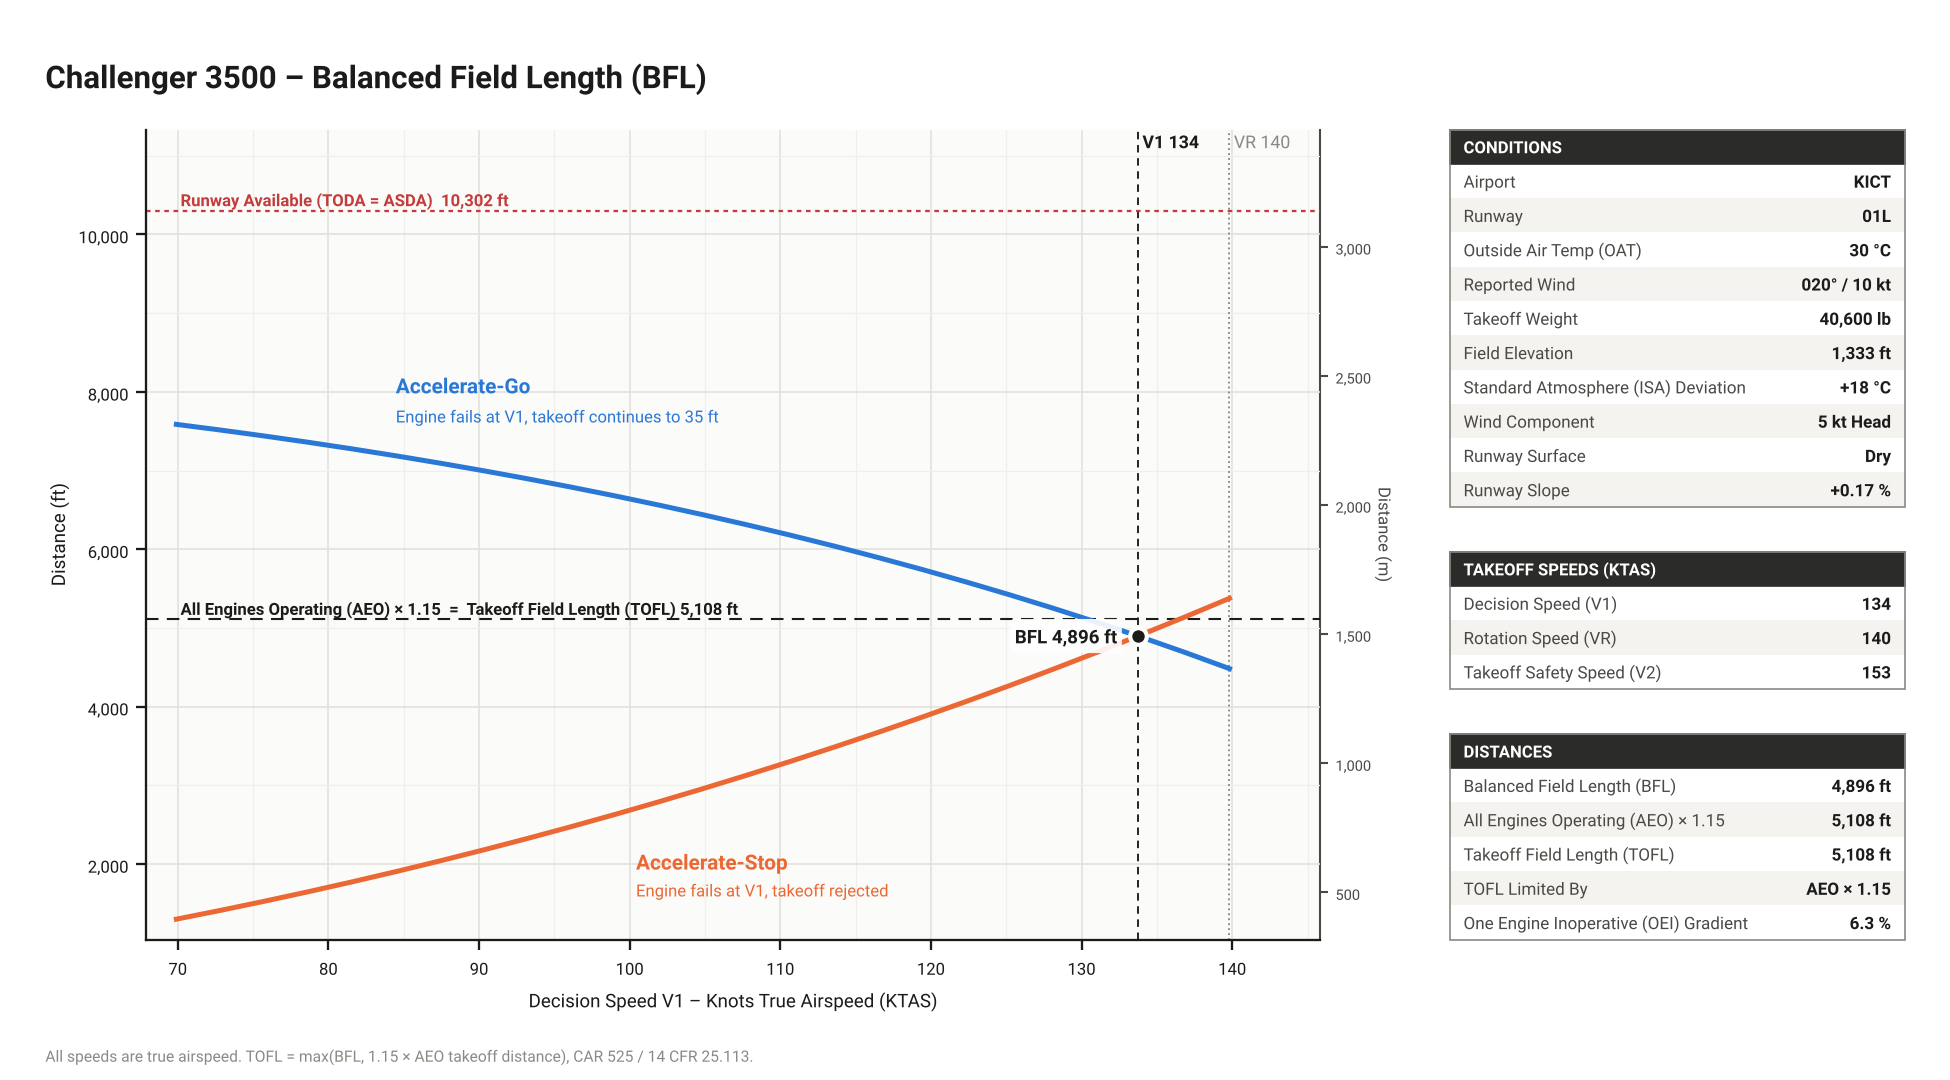
\includegraphics[width=\linewidth]{figures/bfl_example_Challenger_3500.png}
\caption{Challenger 3500: Balanced Field Length (BFL) for this example.}\end{figure}
\subsection{Step 8: Landing}
Landing at MLW on the same runway, no reverse thrust credit (\eqref{eq:vref}--\eqref{eq:ldr}):
\begin{align*}
V_{S0} &= \sqrt{\frac{2\times\num{151907}}{\num{1.1094}\times\num{48.50}\times\num{2.30}}} = \SI{49.55}{m/s} = \SI{96.3}{kt}\\
V_\text{REF} &= \num{1.30}\,V_{S0} = \SI{125.2}{kt}, \qquad V_\text{TD} = \num{1.15}\,V_{S0} = \SI{110.8}{kt}\\
s_\text{air} &= \frac{\num{15.24}}{\tan\ang{3}}\times\frac{\num{64.41} - \num{2.57}}{\num{64.41}} = \SI{279.2}{m}\\
s_\text{free} &= (\num{56.98} - \num{2.57})\times\num{3} = \SI{163.2}{m}\\
s_\text{brake} &= \SI{367.7}{m} \quad\text{(\eqref{eq:eom-brake} integrated to rest, \num{13.6}\,s)}\\
\text{LD} &= \num{279.2} + \num{163.2} + \num{367.7} = \SI{810.1}{m} = \SI{2658}{ft}
\\ \text{LDR} &= \frac{\num{810.1}}{0.6} = \SI{1350.2}{m} = \SI{4430}{ft}
\end{align*}
\subsection{Step 9: Runway Check}
\begin{table}[H]\centering\small
\begin{tabular}{@{}lrlrrl@{}}\toprule \textbf{Required} & \textbf{ft} & \textbf{Available} & \textbf{ft} & \textbf{Margin (ft)} & \textbf{Result}\\\midrule
Takeoff Field Length (TOFL) & \num{5108} & TODA & \num{10302} & \num{5194} & OK\\
Accelerate-Stop Distance (ASD) & \num{4896} & ASDA & \num{10302} & \num{5406} & OK\\
Landing Distance Required (LDR) & \num{4430} & LDA & \num{10302} & \num{5872} & OK\\
\bottomrule\end{tabular}\caption{Challenger 3500: runway check, KICT runway 01L.}\end{table}


% =============================================================================
\clearpage
\section{Example B: Cirrus SR22T}\label{sec:exB}
% =============================================================================
% Generated by make_examples.py from the model. Do not edit by hand.
\subsection{Inputs}
Table~\ref{tab:in-Cirrus_SR22T} lists the aircraft data and the day's conditions. The example uses Wichita Dwight D. Eisenhower National (KICT) runway 01L.
\begin{table}[H]\centering\small
\begin{tabular}{@{}ll@{}}\toprule \textbf{Input} & \textbf{Value}\\\midrule
Maximum takeoff weight (MTOW) & \SI{3600}{lb} = \SI{1632.9}{kg}\\
Maximum landing weight (MLW) & \SI{3600}{lb} = \SI{1632.9}{kg}\\
Reference wing area, $S$ & \SI{13.46}{m^2} (\SI{144.9}{ft^2})\\
$C_{D_0}$ / $k$ & \num{0.027} / \num{0.045}\\
$C_{L,\max}$ takeoff / landing & \num{1.60} / \num{2.04}\\
$C_{L,\text{gnd}}$ & \num{0.40}\\
$\mu_\text{roll}$ / $\mu_\text{brake}$ & \num{0.04} / \num{0.40}\\
Sea-level static thrust, $T_\text{SLS}$ & \SI{3580}{N} (\SI{805}{lbf})\\
Number of engines, $N_e$ & 1\\
Maximum power, $P_\text{max}$ & \SI{234.9}{kW} (\SI{315}{hp})\\
Propeller efficiency, $\eta_p$ & \num{0.72}\\
Turbocharger critical altitude & \SI{25000}{ft}\\
Field elevation, $h$ & \SI{1333}{ft} = \SI{406.3}{m}\\
Outside air temperature (OAT) & \SI{30}{degreeCelsius}\\
Reported wind & \ang{20} / \SI{10}{kt}\\
Runway true heading & \ang{20}\\
Runway slope (direction of travel) & \num{0.165}\,\%\\
Runway condition & Dry\\
TODA = ASDA / LDA & \SI{10302}{ft} / \SI{10302}{ft}\\
\bottomrule\end{tabular}\caption{Cirrus SR22T: example inputs.}\label{tab:in-Cirrus_SR22T}\end{table}
\subsection{Step 1: Atmosphere}
Standard temperature at the field elevation, then the ISA deviation from the OAT (\eqref{eq:isa-temp} and \eqref{eq:isa-dev}):
\begin{align*}
\Theta_\text{std} &= \num{288.15} - \num{0.0065}\times\num{406.3} = \SI{285.51}{K}\\
\Delta T &= \num{30.0} - (\num{285.51} - \num{273.15}) = \SI{17.64}{degreeCelsius}\quad\text{(ISA }+17.6\text{)}
\end{align*}
Pressure, temperature, density, density ratio and speed of sound (\eqref{eq:isa-p}--\eqref{eq:isa-a}):
\begin{align*}
p &= \num{101325}\left(\frac{\num{285.51}}{\num{288.15}}\right)^{\num{5.2559}} = \SI{96538}{Pa}\\
\Theta &= \num{285.51} + \num{17.64} = \SI{303.15}{K}\\
\rho &= \frac{\num{96538}}{\num{287.05}\times\num{303.15}} = \SI{1.1094}{kg/m^3}\\
\sigma &= \frac{\num{1.1094}}{\num{1.225}} = \num{0.9056}\\
a &= \sqrt{\num{1.4}\times\num{287.05}\times\num{303.15}} = \SI{349.0}{m/s}
\end{align*}
\subsection{Step 2: Wind}
Runway components (\eqref{eq:wind-hw}--\eqref{eq:wind-xw}), then the regulatory factor \eqref{eq:wind-perf}:
\begin{align*}
V_w &= \num{10}\cos(\ang{20} - \ang{20}) = \SI{10.0}{kt}\qquad V_x = \num{10}\sin(\ang{0}) = \SI{0.0}{kt}\\
V_{w,\text{perf}} &= \num{0.5}\times\num{10.0} = \SI{5.0}{kt} = \SI{2.57}{m/s}
\end{align*}
All following steps use the performance headwind of \SI{5.0}{kt}.
\subsection{Step 3: Weight and Takeoff Speeds}
\begin{align*}
W &= m\,g_0 = \num{1632.9}\times\num{9.80665} = \SI{16014}{N}\\
V_{S1} &= \sqrt{\frac{2\times\num{16014}}{\num{1.1094}\times\num{13.46}\times\num{1.60}}} = \SI{36.61}{m/s} = \SI{71.2}{kt}\\
V_R &= \num{1.10}\,V_{S1} = \SI{40.27}{m/s} = \SI{78.3}{kt}\\
V_2 &= \num{1.20}\,V_{S1} = \SI{43.93}{m/s} = \SI{85.4}{kt}\\
V_\text{TR} &= \num{1.15}\,V_{S1} = \SI{42.10}{m/s} = \SI{81.8}{kt}
\end{align*}
\subsection{Step 4: Forces on the Ground Roll}
Thrust \eqref{eq:T-prop}, turbocharged below its critical altitude so the power is not reduced ($\sigma_P = 1$):
\begin{equation*}
T(V) = \min\left(\num{1.0000}\times\num{3580},\ \frac{\num{0.72}\times\num{1.0000}\times\num{234895}}{V}\right)
\end{equation*}
\Needspace{16\baselineskip}
Forces at brake release and at $V_R$ (\eqref{eq:eom-accel}, $C_L = C_{L,\text{gnd}} = \num{0.40}$, slope force $W\sin\theta$):
\begin{table}[H]\centering\small
\begin{tabular}{@{}lrr@{}}\toprule \textbf{Quantity} & \textbf{At $V_\text{TAS} = V_w$ (start)} & \textbf{At $V_R$}\\\midrule
Dynamic pressure $q$ (Pa) & \num{3.7} & \num{899.6}\\
Lift $L$ (N) & \num{20} & \num{4844}\\
Drag $D$ (N) & \num{2} & \num{414}\\
Thrust $T$ (N) & \num{3580} & \num{3580}\\
Rolling friction $\mu_\text{roll}(W-L)$ (N) & \num{640} & \num{447}\\
Slope force $W\sin\theta$ (N) & \num{26} & \num{26}\\
Acceleration $a$ (\si{m/s^2}) & \num{1.783} & \num{1.649}\\
\bottomrule\end{tabular}\caption{Cirrus SR22T: forces on the ground roll.}\end{table}
\subsection{Step 5: Ground Roll by Numerical Integration}
Equation~\eqref{eq:eom-accel} is integrated with RK45 from rest until $V_\text{TAS} = V_R$. Selected points from the solver:
\begin{table}[H]\centering\small
\begin{tabular}{@{}rrrr@{}}\toprule \textbf{$t$ (s)} & \textbf{$V_\text{TAS}$ (kt)} & \textbf{$a$ (\si{m/s^2})} & \textbf{$s$ (ft)}\\\midrule
\num{0.0} & \num{5.0} & \num{1.783} & \num{0}\\
\num{2.1} & \num{12.3} & \num{1.781} & \num{13}\\
\num{6.1} & \num{26.1} & \num{1.769} & \num{109}\\
\num{10.1} & \num{39.8} & \num{1.749} & \num{298}\\
\num{14.1} & \num{53.3} & \num{1.721} & \num{579}\\
\num{18.1} & \num{66.5} & \num{1.686} & \num{949}\\
\midrule \num{21.73} & \num{78.3} ($V_R$) & \num{1.649} & \num{1361}\\
\bottomrule\end{tabular}\caption{Cirrus SR22T: ground-roll time history (RK45 output).}\end{table}
Rotation for $t_\text{rot}$ \eqref{eq:s-rot}:
\begin{align*}
s_\text{rot} &= (\num{40.27} - \num{2.57})\times\num{1} = \SI{37.7}{m}\\
s_\text{ground} &= \num{414.9} + \num{37.7} = \SI{452.6}{m} = \SI{1485}{ft}
\end{align*}
\subsection{Step 6: Air Distance to the Screen Height}
Climb at $V_2$ with lift equal to weight (\eqref{eq:cl-climb}--\eqref{eq:sin-gamma}); screen height \SI{50}{ft} = \SI{15.24}{m}:
\begin{align*}
q_{V_2} &= \tfrac12\times\num{1.1094}\times\num{43.93}^2 = \SI{1070.6}{Pa}, \qquad C_{L,\text{climb}} = \frac{\num{16014}}{\num{1070.6}\times\num{13.46}} = \num{1.111}\\
D &= \num{1070.6}\times\num{13.46}\times(\num{0.027} + \num{0.045}\times\num{1.111}^2) = \SI{1190}{N}, \qquad T = \SI{3580}{N}\\
\sin\gamma &= \frac{\num{3580} - \num{1190}}{\num{16014}} = \num{0.1493}, \qquad \gamma = \SI{0.1498}{rad}, \qquad \text{gradient} = \num{15.1}\,\%
\end{align*}
Transition arc (\eqref{eq:R-tr}--\eqref{eq:h-tr}):
\begin{align*}
R_\text{TR} &= \frac{\num{42.10}^2}{\num{9.807}\times(\num{1.2} - 1)} = \SI{903.8}{m}\\
h_\text{TR} &= \num{903.8}\,(1 - \cos \num{0.1498}) = \SI{10.12}{m}
\end{align*}
Since $h_\text{TR} < h_\text{scr}$, the arc is followed by a steady climb \eqref{eq:s-air-climb}:
\begin{equation*}
s_\text{air} = \num{903.8}\sin \num{0.1498} + \frac{\num{15.24} - \num{10.12}}{\tan \num{0.1498}} = \num{134.9} + \num{33.9} = \SI{168.8}{m}
\end{equation*}
Corrected for wind \eqref{eq:s-air-wind}, then the takeoff distance \eqref{eq:tod}:
\begin{align*}
s_\text{air} &= \num{168.8}\times\frac{\num{42.10} - \num{2.57}}{\num{42.10}} = \SI{158.5}{m}\\
\text{TOD}_\text{AEO} &= \num{452.6} + \num{158.5} = \SI{611.1}{m} = \SI{2005}{ft}
\end{align*}
\subsection{Step 7: Engine-Failure Case}
The aircraft has one engine, so there is no accelerate-go case and no balanced field length. The required takeoff distance is the all-engines TOD.
\subsection{Step 8: Landing}
Landing at MLW on the same runway, no reverse thrust credit (\eqref{eq:vref}--\eqref{eq:ldr}):
\begin{align*}
V_{S0} &= \sqrt{\frac{2\times\num{16014}}{\num{1.1094}\times\num{13.46}\times\num{2.04}}} = \SI{32.42}{m/s} = \SI{63.0}{kt}\\
V_\text{REF} &= \num{1.30}\,V_{S0} = \SI{81.9}{kt}, \qquad V_\text{TD} = \num{1.15}\,V_{S0} = \SI{72.5}{kt}\\
s_\text{air} &= \frac{\num{15.24}}{\tan\ang{3}}\times\frac{\num{42.15} - \num{2.57}}{\num{42.15}} = \SI{273.1}{m}\\
s_\text{free} &= (\num{37.29} - \num{2.57})\times\num{2} = \SI{69.4}{m}\\
s_\text{brake} &= \SI{171.9}{m} \quad\text{(\eqref{eq:eom-brake} integrated to rest, \num{9.5}\,s)}\\
\text{LD} &= \num{273.1} + \num{69.4} + \num{171.9} = \SI{514.4}{m} = \SI{1688}{ft}
\end{align*}
\subsection{Step 9: Runway Check}
\begin{table}[H]\centering\small
\begin{tabular}{@{}lrlrrl@{}}\toprule \textbf{Required} & \textbf{ft} & \textbf{Available} & \textbf{ft} & \textbf{Margin (ft)} & \textbf{Result}\\\midrule
Takeoff Distance (TOD) & \num{2005} & TODA & \num{10302} & \num{8297} & OK\\
Takeoff ground roll & \num{1485} & TORA & \num{10302} & \num{8817} & OK\\
Landing Distance (LD) & \num{1688} & LDA & \num{10302} & \num{8614} & OK\\
\bottomrule\end{tabular}\caption{Cirrus SR22T: runway check, KICT runway 01L.}\end{table}


% =============================================================================
\section{Assumptions and Limitations}
% =============================================================================
\begin{itemize}
\item Engine failure at $V_\text{EF} = V_1$, with no recognition delay before $V_1$; VMCG not checked.
\item Fixed V-speed ratios ($V_R = 1.1V_{S1}$, $V_2 = 1.2V_{S1}$); no separate minimum-unstick speed (VMU) or liftoff speed (VLOF) schedule.
\item Wet runway modelled only as halved braking friction; the Part~25 wet-runway takeoff rules are not modelled.
\item OEI gradient reported gear-down at $V_2$; second-segment climb and weight, altitude and temperature (WAT) limits not computed.
\item Idle thrust taken as zero when braking; brake energy limits ignored.
\item Field elevation treated as pressure altitude; turbocharged power taken as independent of temperature below the critical altitude.
\item Declared distances approximated from runway length and displaced thresholds.
\item Aircraft aerodynamic coefficients are estimates. For each aircraft one value is calibrated to published data: $C_{L,\max}$ with takeoff flaps for the Challenger 3500 (to its \SI{4835}{ft} takeoff field length \cite{BBD-CL3500}) and the static thrust for the SR22T (to its \SI{1517}{ft} ground roll \cite{AOPA}).
\end{itemize}

% =============================================================================
\addcontentsline{toc}{section}{References}
\begin{thebibliography}{99}\raggedright
\bibitem{RAYMER} D.~P. Raymer, \emph{Aircraft Design: A Conceptual Approach}, 6th~ed. Reston, VA, USA: AIAA, 2018.
\bibitem{NIST-811} A. Thompson and B.~N. Taylor, ``Guide for the use of the International System of Units (SI),'' NIST, Gaithersburg, MD, USA, Spec. Publ. 811, 2008.
\bibitem{ANDERSON-ITF} J.~D. Anderson, \emph{Introduction to Flight}, 8th~ed. New York, NY, USA: McGraw-Hill, 2016.
\bibitem{ICAO-7488} International Civil Aviation Organization, \emph{Manual of the ICAO Standard Atmosphere}, Doc~7488/3, 3rd~ed. Montr\'eal, QC, Canada: ICAO, 1993.
\bibitem{14CFR23} \emph{Airworthiness Standards: Normal Category Airplanes}, 14 C.F.R. Part~23.
\bibitem{14CFR25} \emph{Airworthiness Standards: Transport Category Airplanes}, 14 C.F.R. Part~25.
\bibitem{CAR525} Transport Canada, \emph{Canadian Aviation Regulations}, Airworthiness Manual Ch.~525, \emph{Transport Category Aeroplanes}.
\bibitem{ANDERSON-APD} J.~D. Anderson, \emph{Aircraft Performance and Design}. New York, NY, USA: McGraw-Hill, 1999.
\bibitem{GUDMUNDSSON} S. Gudmundsson, \emph{General Aviation Aircraft Design: Applied Methods and Procedures}. Oxford, U.K.: Butterworth-Heinemann, 2014.
\bibitem{FILIPPONE} A. Filippone, \emph{Advanced Aircraft Flight Performance}. Cambridge, U.K.: Cambridge Univ. Press, 2012.
\bibitem{AIRBUS-GTG} Airbus, ``Getting to grips with aircraft performance,'' Flight Operations Support \& Line Assistance, Blagnac, France, 2002.
\bibitem{OJHA} S.~K. Ojha, \emph{Flight Performance of Aircraft}. Washington, DC, USA: AIAA, 1995.
\bibitem{TORENBEEK} E. Torenbeek, \emph{Synthesis of Subsonic Airplane Design}. Delft, The Netherlands: Delft Univ. Press, 1982.
\bibitem{MAIR-BIRDSALL} W.~A. Mair and D.~L. Birdsall, \emph{Aircraft Performance}. Cambridge, U.K.: Cambridge Univ. Press, 1992.
\bibitem{14CFR121} \emph{Landing Limitations: Destination Airports}, 14 C.F.R. \S121.195.
\bibitem{ICAO-A14} International Civil Aviation Organization, \emph{Annex 14 to the Convention on International Civil Aviation: Aerodromes}, vol.~I. Montr\'eal, QC, Canada: ICAO.
\bibitem{OURAIRPORTS} OurAirports, ``Runway data.'' [Online]. Available: https://ourairports.com. Accessed: Oct.~21, 2026.
\bibitem{BBD-CL3500} Bombardier, ``Challenger 3500 factsheet,'' Montr\'eal, QC, Canada, 2024.
\bibitem{AOPA} Aircraft Owners and Pilots Association, ``Aircraft guide: Bombardier Challenger 350; Cirrus SR22T.'' [Online]. Available: https://www.aopa.org
\end{thebibliography}

% =============================================================================
\appendix
\section{Model Constants}
% =============================================================================
\begin{table}[H]
\centering
\small
\begin{tabular}{@{}llll@{}}
\toprule
\textbf{Constant} & \textbf{Value} & \textbf{Meaning} & \textbf{Source}\\
\midrule
$V_R / V_{S1}$ & 1.1 & Rotation speed ratio & \cite{RAYMER}\\
$V_2 / V_{S1}$ & 1.2 & Takeoff safety speed ratio & \cite{RAYMER}, \cite{14CFR25}\\
$V_\text{TR} / V_{S1}$ & 1.15 & Transition speed ratio & \cite{RAYMER}\\
$n$ & 1.2 & Load factor in the transition arc & \cite{RAYMER}\\
$t_\text{rot}$ & \SI{1}{s} / \SI{3}{s} & Rotation time, prop / jet & \cite{RAYMER}\\
$h_\text{scr}$, takeoff & \SI{50}{ft} / \SI{35}{ft} & Screen height, Part 23 / Part 25 & \cite{14CFR23}, \cite{14CFR25}\\
$h_\text{scr}$, landing & \SI{50}{ft} & Screen height, all aircraft & \cite{14CFR25}\\
$t_\text{stop}$ & \SI{2}{s} & Allowance at V1 before stopping & \cite{14CFR25} \S25.109\\
AEO factor & 1.15 & TOFL $\ge 1.15\,\text{TOD}_\text{AEO}$ & \cite{14CFR25} \S25.113\\
$V_\text{REF} / V_{S0}$ & 1.3 & Landing reference speed ratio & \cite{RAYMER}\\
$V_\text{TD} / V_{S0}$ & 1.15 & Touchdown speed ratio & \cite{RAYMER}\\
Glideslope & \ang{3} & Approach path angle & \cite{AIRBUS-GTG}\\
$t_\text{free}$ & \SI{2}{s} / \SI{3}{s} & Free roll, prop / jet & \cite{RAYMER}\\
Reverser cutoff & \SI{60}{kt} & Reversers stowed below & \cite{AIRBUS-GTG}\\
LDR factor & $1/0.6$ & Landing within 60\% of runway & \cite{14CFR121} \S121.195\\
Wet LDR factor & 1.15 & Wet runway & \cite{14CFR121} \S121.195\\
Wind factors & 0.5 / 1.5 & Headwind / tailwind & \cite{14CFR25} \S25.105\\
Wet braking & $0.5\,\mu_\text{brake}$ & Wet runway friction & simplified\\
Integration step & \SI{0.5}{s} & RK45 maximum step & --\\
\bottomrule
\end{tabular}
\caption{Constants used in the model.}\label{tab:constants}
\end{table}

\end{document}
